\begin{section}{Results}
  \label{sec:results}
  We now present the results of a simulation of $128^3$ neutrinos 
with mass 0.2eV and $64^3$ dark matter particles. The simulation 
is done in a box of size $500 \mpch{}$. As noted above, initial 
conditions for dark matter particles are produced at $z=100$ 
whereas neutrinos are introduced at $z=10$. We take cosmological 
parameters which are in line with the most recent Planck results 
\cite{bib:Planck2015}: $h=0.67,\, \Omega_b=0.05, \Omega_c=0.27, 
\sigma_8=0.83,\, n_s=0.96 $, and

\begin{equation}
  \Omega_\nu = \frac{m_\nu}{93.14 h^2}
\end{equation}
We assume a flat universe and so set $\Omega_\Lambda=1-\Omega_m=1-\Omega_b-\Omega_c-\Omega_\nu$.

\par The dimensionless density power spectra of the four velocity 
bins are depicted in Fig. \ref{fig:denpowerfig}. We find that 
neutrinos with smaller initial velocities have greater power at all scales 
with the difference in power between the velocity bins increasing at smaller scales. 
This is to be expected as less energetic neutrinos are more easily trapped 
in potential wells and thus tend to cluster, resulting in an overdensity at all -
but particularly small - scales relative to more energetic neutrinos. 
This also results in the power spectra of the neutrinos with the 
smallest initial velocities deviating the most from linear theory predictions. 

\par The velocity power spectra are shown in Fig. \ref{fig:velpowerfig}. 
We compare the power spectra of the actual velocity field and the reconstructed
fields using a linear and a non-linear transfer function. 
A similar pattern is evident as neutrinos with smaller initial velocity have
greater power at all scales. This is reasonable as the velocities of 
less energetic neutrinos are more likely to be correlated as their 
velocities are more easily perturbed through gravitational interaction. 

\begin{figure}[htbp]
  \begin{center}
    \includegraphics[width=0.5\textwidth]{./figures/DensityPowerSpectra/denpower.pdf}
    \caption{Density power spectra of the four neutrino velocity bins
	      at z=0 (solid lines). Also plotted are the power spectra predicted by
	      linear theory (dashed lines).}
    \label{fig:denpowerfig}
  \end{center}
\end{figure}

\begin{figure}[htbp]
  \begin{center}
    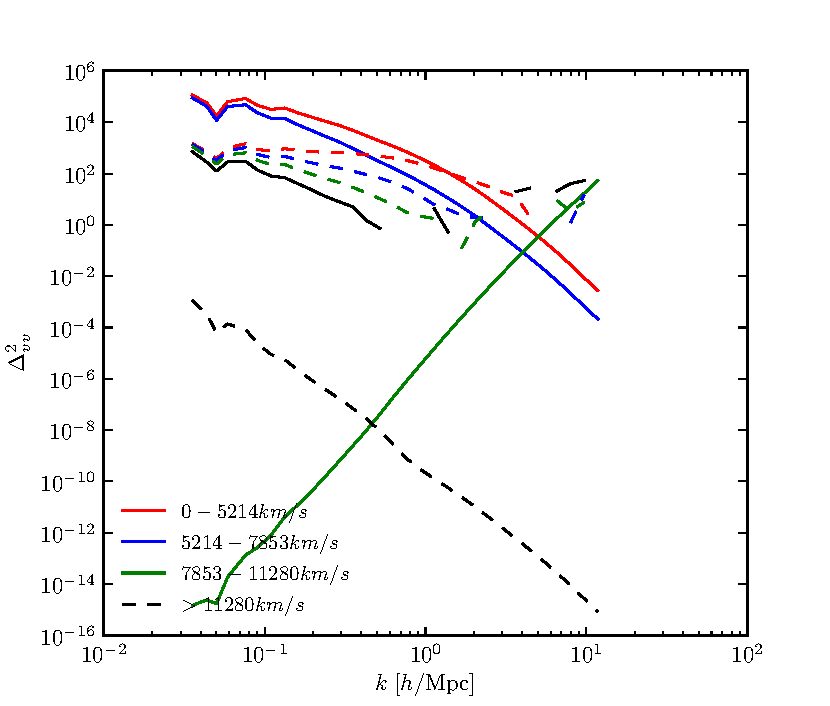
\includegraphics[width=0.5\textwidth]{./figures/VelPowerSpectra/velpower.pdf}
    \caption{Velocity power spectra of the four neutrino velocity
	      bins at z=0 (solid lines) compared with the linear (dashed lines) 
	      and non-linear (dash-dot lines) reconstructed velocity power spectra.}
    \label{fig:velpowerfig}
  \end{center}
\end{figure}

\begin{table}[h]
  \caption{Percentages of neutrinos which began in bin $Q_i$ at $z=10$ 
	   and ended in bin $Q_j '$ at $z=0$.}
  \label{tab:binswitch}
  \begin{tabular}{cc|cccc}
   &  & \multicolumn{4}{l}{$z=0$} \\
  \multirow{5}{*}{\rotatebox[origin=c]{90}{$z=10$}} &  & $Q_1 '$ & $Q_2 '$ & $Q_3 '$ & $Q_4 '$ \\\hline
   & $Q_1$ & 58.9 & 29.2 & 10.0 & 1.8  \\
   & $Q_2$ & 32.8 & 39.4 & 23.8 & 4.0 \\
   & $Q_3$ & 8.2 & 28.4 & 45.5 & 17.8 \\
   & $Q_4$ & 0.2 & 2.9 & 20.6 & 76.3 \\\hline
  \end{tabular}
\end{table}

\par Also of interest is how the velocities of the individual neutrinos change between
$z=10$ and $z=0$. At $z=0$ we again divide the neutrinos into four bins $Q_i '$ based 
on their velocity, each containing an equal number of particles. Table \ref{tab:binswitch} 
indicates what percentage of particles beginning in a bin $Q_i$ at $z=10$ end in a 
bin $Q_j$ at $z=0$. Evidently, neutrinos with a very small or large initial 
velocity (i.e. those initially in bins $Q_1$ and $Q_4$) are more likely to remain 
in the same bin. This seems reasonable as neutrinos with small initial velocities 
will likely remain trapped in potential wells whereas those with large initial velocities 
are likely to have their trajectories only slightly perturbed via gravitational 
interaction.


\par Lastly, we calculate the dipole correlation functions using the total 
neutrino density field and the different velocity fields. In particular, 
we consider the actual velocity fields (calculated using the aforementioned 
momentum method) of all the neutrinos and the individual velocity bins, as 
well as the velocity fields reconstructed using the CDM density field. 
Fig. \ref{fig:dipolefig} depicts the dipole correlation 
function calculated using the total neutrino actual and reconstructed velocity fields. 
For $r>5\mpch$, there is little difference between the two dipole functions,
whereas for smaller $r$, the reconstructed dipole is slightly larger.

\par Fig. \ref{fig:reldipolefig} show the dipole correlation function for 
each of the velocity bins. Again, for $r>5\mpch$ there is little 
difference between most of the dipole correlation functions
calculated using the different methods and the velocity bins. However the
$Q_1$ dipole calulated using the CDM reconstruction method is markedly 
smaller than all other dipoles. For smaller $r$, the dipole from the linear 
reconstruction drops far below the dipole of the actual field in $Q_1$, 
whereas in the other bins, the it remains comparable to or becomes slightly 
greater than the dipole from the actual field. For all scales and 
bins, the dipole from the non-linear reconstruction is also comparable 
to or greater thant the dipole from the actual field. Moreover, for small $r$, 
the dipoles for the larger velocity bins begin to dominate the 
smaller velocity bins; this is particularly pronounced in the dipole 
functions produced using the CDM reconstructed velocity fields.

\begin{figure}[tbp]
  \begin{center}
    \includegraphics[width=0.5\textwidth]{./figures/Dipole/alldipolefig.pdf}
    \caption{Dipole correlation function at z=0 calculated 
	      using the actual total neutrino velocity field (solid line) 
	      and the total neutrino velocity field reconstructed using the CDM 
	      density field (dashed line).}
    \label{fig:dipolefig}
  \end{center}
\end{figure}

\begin{figure}[htbp]
  \begin{center}
    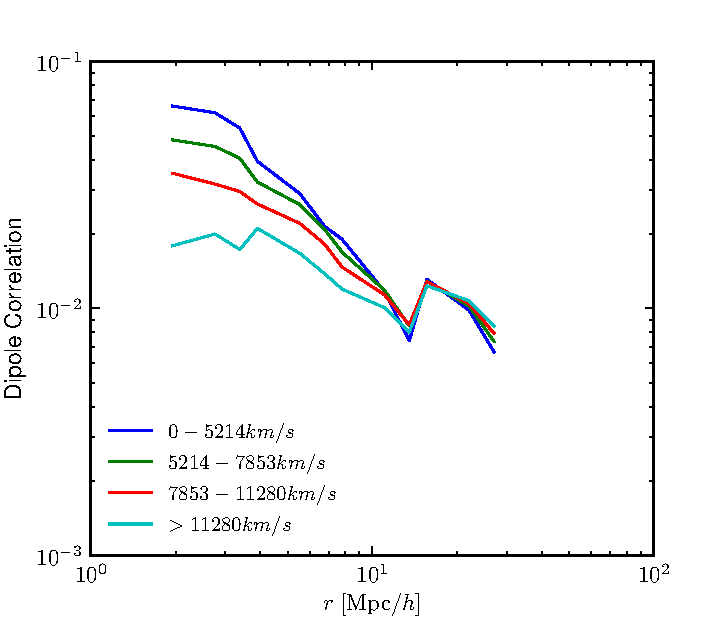
\includegraphics[width=0.5\textwidth]{./figures/Dipole/dipolefig.pdf}
    \caption{Dipole correlation functions for each neutrino
	      velocity bin at z=0 calculated using the actual velocity 
	      field (solid lines), linear reconstructed velocity fields 
	      (dashed lines), and non-linear reconstructed velocity fields 
	      (dash-dot lines).}
    \label{fig:reldipolefig}
  \end{center}
\end{figure}

\end{section}
